% Finite-Elemente (ZHAW) — Beamer-Template
% (Passe Titel/Dozent/Datum nach Bedarf an.)

\documentclass[aspectratio=169,professionalfonts]{beamer}

% --- Sprache/Encoding ---
\usepackage[ngerman]{babel}
\usepackage[T1]{fontenc}
\usepackage[utf8]{inputenc}

% --- Mathe & Grafik ---
\usepackage{amsmath,amssymb,bm}
\usepackage{mathtools}
\usepackage{graphicx}
\usepackage{tikz}
\usetikzlibrary{arrows.meta,positioning,calc,decorations.pathmorphing}

% --- Tabellen/Listen ---
\usepackage{booktabs}
\usepackage{multicol}

% --- Theme/Look ---
\usetheme{Madrid}
\usecolortheme{default}
\setbeamertemplate{navigation symbols}{}

% Fußzeile: Foliennummern
\setbeamertemplate{footline}{%
  \leavevmode%
  \hbox{%
  \begin{beamercolorbox}[wd=.8\paperwidth,ht=2.5ex,dp=1.1ex,left]{author in head/foot}\hspace{1em}\insertshortauthor\hspace{1em}--\hspace{1em}\insertshorttitle\end{beamercolorbox}%
  \begin{beamercolorbox}[wd=.2\paperwidth,ht=2.5ex,dp=1.1ex,right]{date in head/foot}\insertframenumber{} / \inserttotalframenumber\hspace{1em}\end{beamercolorbox}}%
  \vskip0pt%
}

% --- Metadaten ---
\title[FEM]{Finite Elemente Methode}
\subtitle{Vorlesung}
\author[ZHAW]{Sebastian Domaschke}
\institute[ZHAW]{Zürcher Hochschule für Angewandte Wissenschaften (ZHAW)}
\date{Frühlingssemester 2026}
\titlegraphic{
\includegraphics[height=1.2cm]{../Grafiken/logo.pdf}}

% --- Nützliche Makros ---
\newcommand{\R}{\mathbb{R}}
\newcommand{\dd}{\,\mathrm{d}}
\newcommand{\grad}{\nabla}
\newcommand{\K}{\mathbf{K}}
\newcommand{\fvec}{\mathbf{f}}
\newcommand{\uvec}{\mathbf{u}}

\begin{document}

% Titelfolie
\begin{frame}
  \titlepage
\end{frame}



\begin{frame}{Übergeordnetes Lernziel 1}
  \centering
  {\LARGE FEM mittels Softwaretool \textbf{Abaqus}}
\end{frame}

\begin{frame}{Wiederholung: Symmetrie, ESZ und EVZ}
  \small
  \begin{itemize}
    \item Wiederholung: Symmetriebedingungen sowie ESZ und EVZ (gemäss Folien auf Moodle).
    \item VL01-04 \emph{Abaqus Intro (de)}:
      \href{https://moodle.zhaw.ch/pluginfile.php/121654/mod_resource/content/2/VL01-04_Abaqus_Intro_de_v01.pdf}{VL01-04\_Abaqus\_Intro\_de\_v01.pdf}
    \item Abaqus Kurzanleitung (Moodle):
      \href{https://moodle.zhaw.ch/pluginfile.php/121648/mod_resource/content/4/Abaqus_Kurzanleitung_R2024.pdf}{Abaqus\_Kurzanleitung\_R2024.pdf}
  \end{itemize}
\end{frame}

\begin{frame}{Übergeordnetes Lernziel 2}
  \centering
  \begin{minipage}{0.9\linewidth}
    \centering
    {\LARGE  Herleitung / Erklärung FEM\\[0.6em]}
    {\Large bestehend aus 1D-Elementen (Federn, Stäben, Balken)\\[0.4em]}
    {\Large mittels \textbf{Matrixsteifigkeitsmethode}}
  \end{minipage}
\end{frame}

\begin{frame}{Lernziele Vorlesung}
  \small
  Sie können
  \begin{enumerate}
    \item die lokale Elementsteifigkeitsmatrix $\mathbf{k}^e$ ($f^e=\mathbf{k}^eu^e$) für ein Feder und ein Stabelement aufstellen,
    \item unterscheiden zwischen
      \begin{itemize}
        \item lokalen Elementverschiebungen $u_i^e$ / Elementkräften $f_i^e$ ($i=1,2$),
        \item globalen Elementverschiebungen $U_j^e$ / Elementkräften $F_j^e$ ($j=1,\dots,4$),
        \item Strukturverschiebungen $U_l$ / Strukturkräften $F_l$ ($l=1,\dots,n$),
      \end{itemize}
    \item Elementverschiebungen und Elementkräfte vom lokalen ins globale System transformieren.
  \end{enumerate}
\end{frame}


% Motivation
\begin{frame}{Motivation}
  \begin{columns}[T,onlytextwidth]
    \begin{column}{0.49\textwidth}
      \centering
      % TODO: Bild 1 ersetzen
      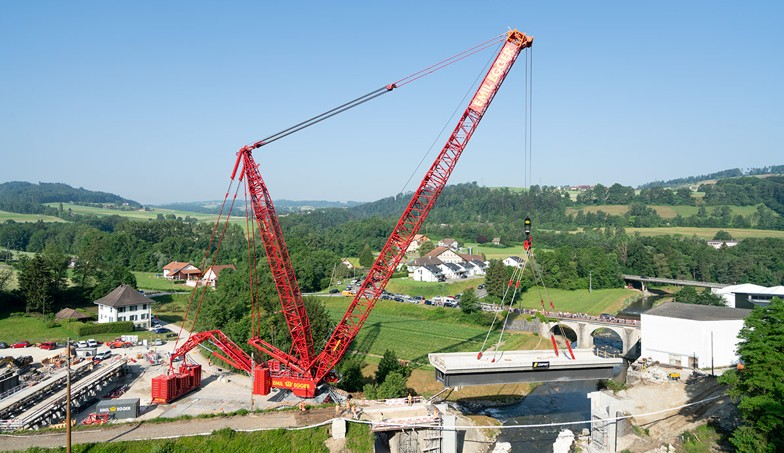
\includegraphics[width=\linewidth,height=0.62\textheight,keepaspectratio]{../Grafiken/Liebherr.jpg}

      \vspace{0.2em}
      {\footnotesize Liebherr LR 11000}
    \end{column}
    \hspace{0.02\textwidth}
    \begin{column}{0.49\textwidth}
      \centering
      % TODO: Bild 2 ersetzen
      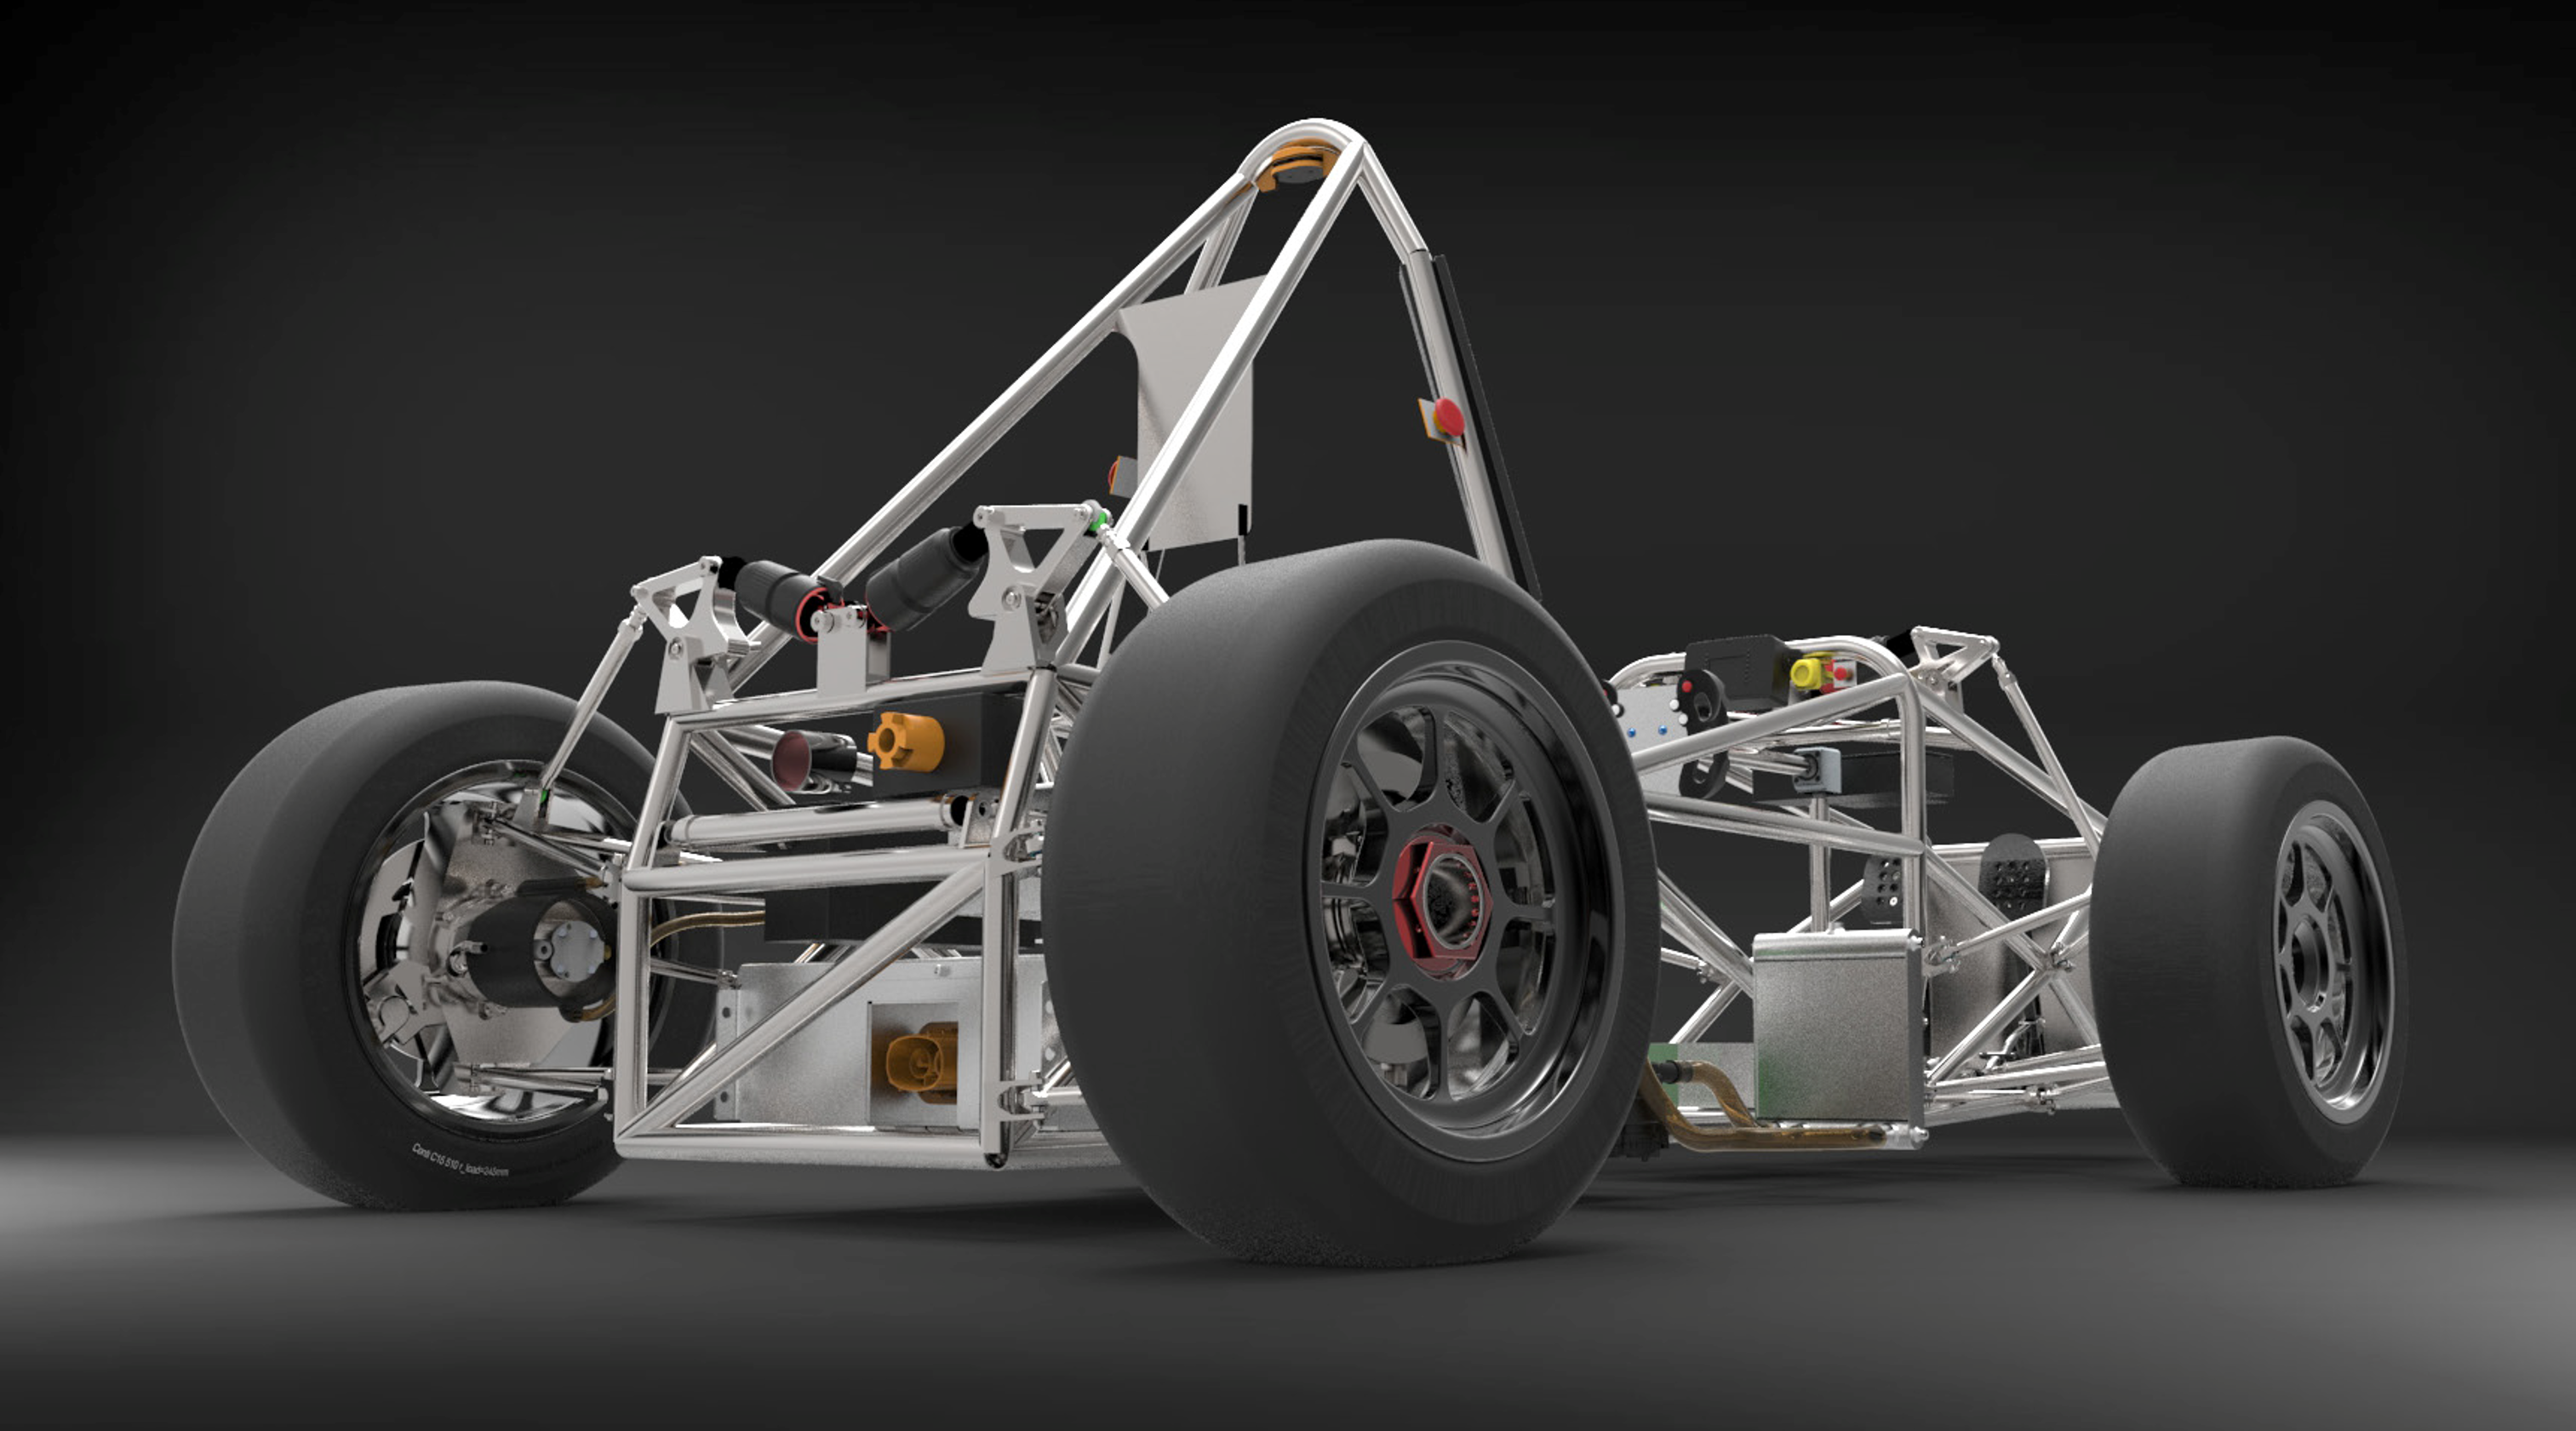
\includegraphics[width=\linewidth,height=0.62\textheight,keepaspectratio]{../Grafiken/FormulaStudent.png}

      \vspace{0.2em}
      {\footnotesize Formula Student}
    \end{column}
  \end{columns}

  \vspace{0.3em}
  \footnotesize
  \footnote{Quellenlinks: (1) \href{https://www.liebherr.com/de/che/produkte/mobil-und-raupenkrane/kundenmagazin/alles-ueber-krane/v-frame.html
\includegraphics[width=0.5\textwidth]{image.png}}{www.liebherr.com}, (2) \href{https://www.inneo.de/files/content/Download/Referenzen/bern-formula-student-106249-20170504.pdf
\includegraphics[width=0.5\textwidth]{image_2.png}}{www.inneo.de}.}
\end{frame}

\begin{frame}{Wiederholgung Physik 3: Kraftgesetz Feder-Element}
  \small
  \begin{columns}[T,onlytextwidth]
    \begin{column}{0.49\textwidth}
      \centering
      \begin{tikzpicture}[scale=0.9,
        spring/.style={decorate, decoration={coil, segment length=4pt, amplitude=3pt}, thick},
        load/.style={red!80!black, very thick, -{Latex[length=3mm]}},
        disp/.style={green!60!black, very thick, -{Latex[length=3mm]}}
      ]
        % Feder
        \draw[load] (-2,1.2) -- (-1.2,1.2) node[above left] {$F$};
        \draw[spring] (-1.2,1.2) -- (1.2,1.2);
        \draw[load] (2,1.2) -- (1.2,1.2) node[above right] {$F$};
        \node at (0,1.55) {$c$};

        % Verschiebungen
        \draw[disp] (-0.55,0.2) -- (-1.6,0.2) node[above] {$x_1$};
        \draw[disp] (0.55,0.2) -- (1.6,0.2) node[above] {$x_2$};

        % l0
        \draw[thick] (-0.55,-0.15) -- (-0.55,0.55);
        \draw[thick] (0.55,-0.15) -- (0.55,0.55);
        \draw[<->] (-0.55,-0.05) -- (0.55,-0.05);
        \node[below] at (0,-0.05) {$l_0$};
      \end{tikzpicture}

      \vspace{0.5em}
      \begin{tabular}{@{}l@{}}
        $\bigcirc\ \ F=c(x_1+x_2)$\\[0.3em]
        $\bigcirc\ \ F=c(x_1-x_2)$\\[0.3em]
        $\bigcirc\ \ F=c(-x_1-x_2)$
      \end{tabular}
    \end{column}

    \begin{column}{0.49\textwidth}
      \centering
      \begin{tikzpicture}[scale=0.9,
        spring/.style={decorate, decoration={coil, segment length=4pt, amplitude=3pt}, thick},
        load/.style={red!80!black, very thick, -{Latex[length=3mm]}},
        disp/.style={green!60!black, very thick, -{Latex[length=3mm]}}
      ]
        % Feder
        \fill ( -1.2,1.2) circle (2pt);
        \fill (  1.2,1.2) circle (2pt);
        \draw[load] (-2,1.2) -- (-1.2,1.2) node[above left] {$F$};
        \draw[spring] (-1.2,1.2) -- (1.2,1.2);
        \draw[load] (1.2,1.2) -- (2,1.2) node[above right] {$F$};
        \node at (0,1.55) {$c$};

        % Verschiebungen
        \draw[disp] (-0.55,0.2) -- (0.2,0.2) node[above] {$x_1$};
        \draw[disp] (0.55,0.2) -- (1.6,0.2) node[above] {$x_2$};

        % l0
        \draw[thick] (-0.55,-0.15) -- (-0.55,0.55);
        \draw[thick] (0.55,-0.15) -- (0.55,0.55);
        \draw[<->] (-0.55,-0.05) -- (0.55,-0.05);
        \node[below] at (0,-0.05) {$l_0$};
      \end{tikzpicture}

      \vspace{0.5em}
      \begin{tabular}{@{}l@{}}
        $\bigcirc\ \ F=c(x_1-x_2)$\\[0.3em]
        $\bigcirc\ \ F=c(x_2-x_1)$\\[0.3em]
        $\bigcirc\ \ F=c(x_2+x_1)$
      \end{tabular}
    \end{column}
  \end{columns}
\end{frame}



\newsavebox{\FachwerkPic}
\sbox{\FachwerkPic}{%
\begin{tikzpicture}[scale=0.95, every node/.style={font=\small},
  disp/.style={draw=green!70!black, very thick, -{Latex[length=3mm]}, green!70!black},
  load/.style={draw=red!80!black, very thick, -{Latex[length=3mm]}, red!80!black},
  member/.style={line width=1.2pt, black},
  joint/.style={circle, fill=black, inner sep=2.2pt},
  elbox/.style={draw, rectangle, inner sep=2pt, fill=white}
]
  % Knoten
  \coordinate (n1) at (0,0);
  \coordinate (n2) at (4,0);
  \coordinate (n3) at (4,3);
  \coordinate (n4) at (8,3);

  % Stäbe (Elemente)
  \draw[member] (n1) -- (n2); % e1
  \draw[member] (n1) -- (n3); % e2
  \draw[member] (n2) -- (n3); % e3
  \draw[member] (n2) -- (n4); % e4
  \draw[member] (n3) -- (n4); % e5

  % Gelenke
  \node[joint] at (n1) {};
  \node[joint] at (n2) {};
  \node[joint] at (n3) {};
  \node[joint] at (n4) {};

  % Knotennummern
  \node[above left] at (n1) {$1$};
  \node[above left] at (n2) {$2$};
  \node[above left] at (n3) {$3$};
  \node[above left] at (n4) {$4$};

  % Elementnummern
  \node[elbox] at (2.0,-0.35) {$1$};
  \node[elbox] at (1.8,1.45) {$2$};
  \node[elbox] at (4.25,1.5) {$3$};
  \node[elbox] at (6.0,1.35) {$4$};
  \node[elbox] at (6.0,3.25) {$5$};

  % Lager
  \draw[line width=1pt] (n1) ++(-0.35,-0.35) -- ++(0.70,0) ;
  \draw[line width=1pt] (n1) ++(-0.35,-0.35) -- (n1);
  \draw[line width=1pt] (n1) ++(0.35,-0.35) -- (n1);
  \foreach \xx in {-0.40,-0.28,...,0.40} {\draw (n1) ++(\xx,-0.35) -- ++(0.12,-0.12);}

  \draw[line width=1pt] (n2) ++(-0.35,-0.35) -- ++(0.70,0) ;
  \draw[line width=1pt] (n2) ++(-0.35,-0.35) -- (n2);
  \draw[line width=1pt] (n2) ++(0.35,-0.35) -- (n2);
  \foreach \xx in {-0.40,-0.28,...,0.40} {\draw (n2) ++(\xx,-0.35) -- ++(0.12,-0.12);}

  % Verschiebungen (grün)
  \draw[disp] (n1) -- ++(1.1,0) node[below right] {$U_1$};
  \draw[disp] (n1) -- ++(0,1.1) node[left] {$U_2$};

  \draw[disp] (n2) -- ++(1.1,0) node[below right] {$U_3$};
  \draw[disp] (n2) -- ++(0,1.1) node[left] {$U_4$};

  \draw[disp] (n3) -- ++(1.1,0) node[above] {$U_5$};
  \draw[disp] (n3) -- ++(0,1.1) node[left] {$U_6$};

  \draw[disp] (n4) -- ++(1.1,0) node[above] {$U_7$};
  \draw[disp] (n4) -- ++(0,1.1) node[left] {$U_8$};

  % Last (rot)
  \draw[load] (n4) -- ++(0,-1.4) node[right] {$F$};

  % Koordinatensystem
  \draw[->,thick] (6.8,0.1) -- ++(1.0,0) node[right] {$X$};
  \draw[->,thick] (6.8,0.1) -- ++(0,1.0) node[above] {$Y$};
\end{tikzpicture}%
}

\begin{frame}{Herleitung lokale Elementsteifigkeitsmatrix Feder / Stab (Tafel)}
\centering



\end{frame}

\begin{frame}{Echte Probleme: Systeme aus mehreren Elementen (z.B. Fachwerk)}
  \centering
  \usebox{\FachwerkPic}
\end{frame}

\begin{frame}{Idee: Assemblierung - Globale Systemsteifigkeit aus Elementsteifigkeiten}
  \centering
  % TODO: Bitte das bereitgestellte Bild als Datei nach \texttt{../Grafiken/Assemblierung-Zyklus.png} hochladen
  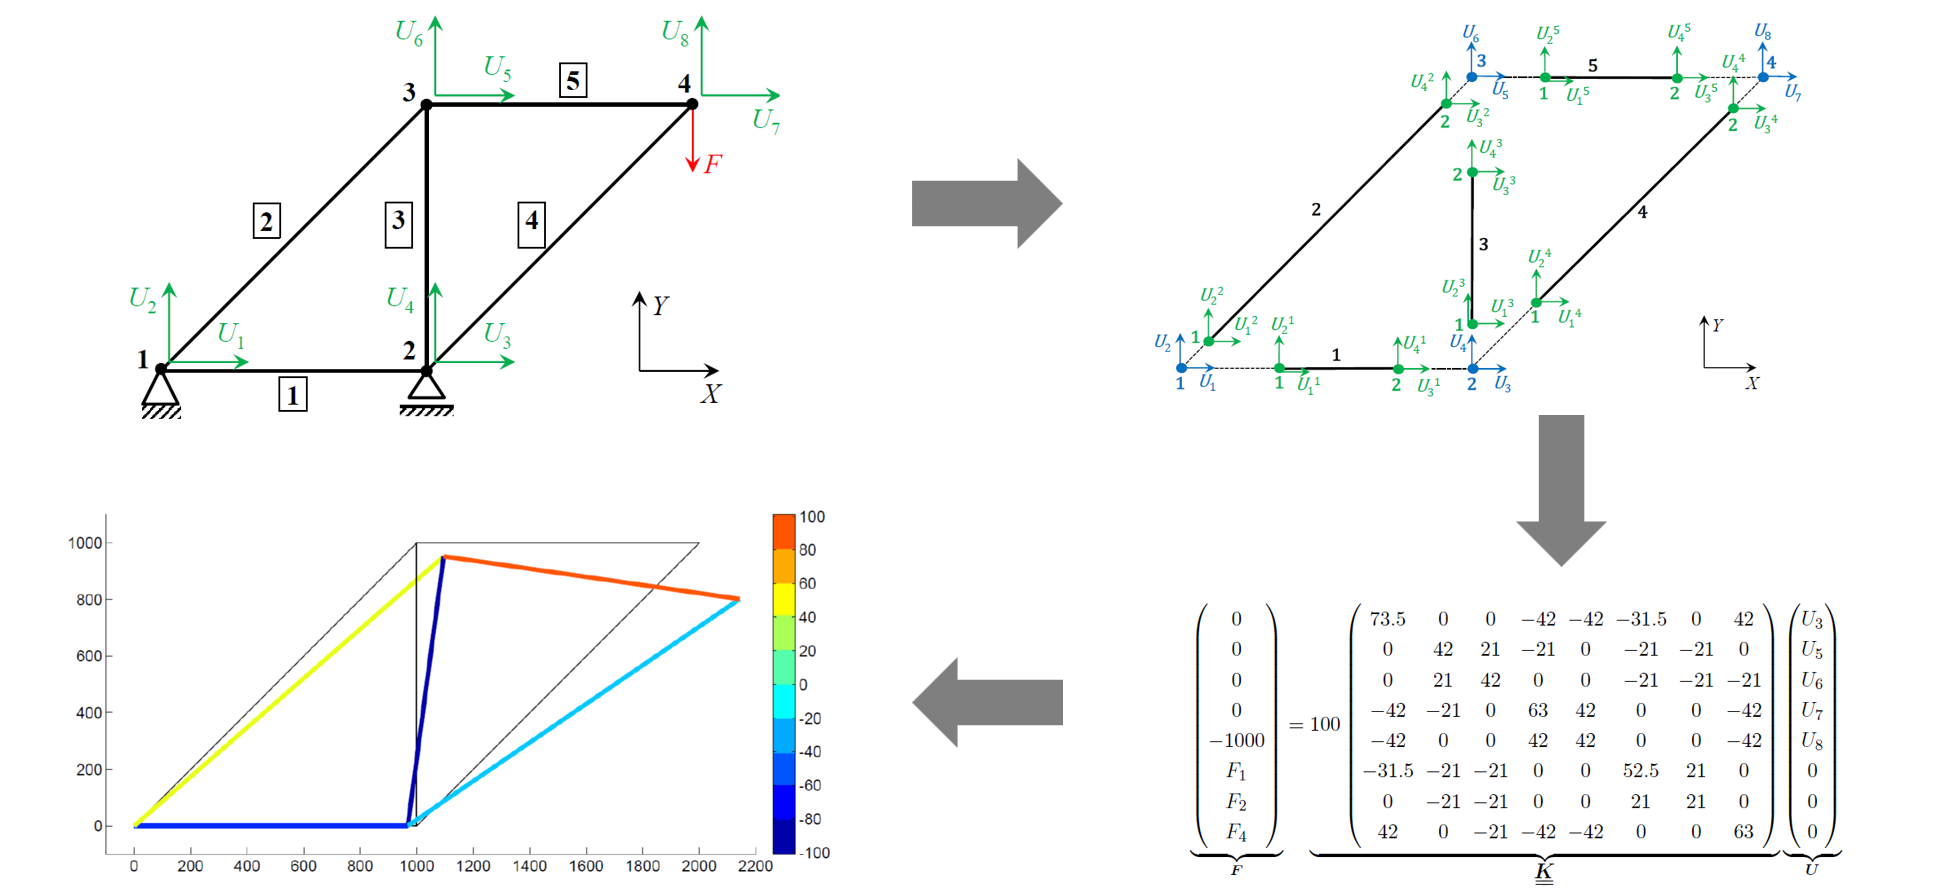
\includegraphics[width=0.98\linewidth,height=0.80\textheight,keepaspectratio]{../Grafiken/Assemblierung-Zyklus.png}
\end{frame}

\begin{frame}{Herleitung globale Elementsteifigkeitsmatrix horizontaler Stab (Tafel)}
\centering
\end{frame}

\begin{frame}{Wichtigste Formeln der Vorlesung (Stab)}
  \small
  \begin{columns}[T,onlytextwidth]
    \begin{column}{0.49\textwidth}
      \begin{flushleft}
        \begin{tikzpicture}[scale=0.90,
          force/.style={red!80!black, very thick, -{Latex[length=3mm]}},
          disp/.style={green!60!black, very thick, -{Latex[length=3mm]}},
          bar/.style={black, line width=2.2pt}
        ]
          % Knoten
          \coordinate (n1) at (0,0);
          \coordinate (n2) at (6,0);

          % Stab
          \draw[bar] (n1) -- (n2);

          % Knotensymbole
          \fill[blue] (n1) circle (2.6pt);
          \fill[blue] (n2) circle (2.6pt);
          \node[blue, above right] at (n1) {1};
          \node[blue, above left] at (n2) {2};

          % Material/Querschnitt
          \node[above] at (3,0.28) {$E^eA^e$};

          % Kräfte (rot)
          \draw[force] (-0.75,0.35) -- (0,0.35) node[above left] {$f_1^e$};
          \draw[force] (6,0.35) -- (6.75,0.35) node[above right] {$f_2^e$};

          % Verschiebungen (grün)
          \draw[disp] (-0.75,-0.35) -- (0,-0.35) node[below left] {$u_1^e$};
          \draw[disp] (6,-0.35) -- (6.75,-0.35) node[below right] {$u_2^e$};

          % Länge
          \draw[thin] (0,0) -- (0,-0.95);
          \draw[thin] (6,0) -- (6,-0.95);
          \draw[<->,thick] (0,-0.95) -- (6,-0.95);
          \node[below] at (3,-0.95) {$L^e$};
        \end{tikzpicture}

        \vspace{0.4em}

        $$\mathbf{f}^e = \mathbf{k}^e\,\mathbf{u}^e$$

        \vspace{0.4em}

        $$\mathbf{k}^e = \frac{E^e A^e}{L^e}
        \begin{pmatrix}
          1 & -1\\
          -1 & 1
        \end{pmatrix}$$
      \end{flushleft}
    \end{column}

    \begin{column}{0.49\textwidth}
      {\color{gray!60}
      \begin{flushleft}
        \begin{tikzpicture}[scale=0.90,
          force/.style={gray!60, very thick, -{Latex[length=3mm]}},
          disp/.style={gray!60, very thick, -{Latex[length=3mm]}},
          spring/.style={gray!60, decorate, decoration={coil, segment length=4pt, amplitude=3pt}, thick}
        ]
          % Knoten
          \coordinate (n1) at (0,0);
          \coordinate (n2) at (6,0);

          % Feder
          \draw[spring] (n1) -- (n2);

          % Knotensymbole
          \fill[gray!60] (n1) circle (2.6pt);
          \fill[gray!60] (n2) circle (2.6pt);
          \node[gray!60, above right] at (n1) {$1$};
          \node[gray!60, above left] at (n2) {$2$};

          % Federkonstante
          \node[gray!60, above] at (3,0.28) {$c$};

          % Kräfte
          \draw[force] (-0.75,0.35) -- (0,0.35) node[above left] {$f_1^e$};
          \draw[force] (6,0.35) -- (6.75,0.35) node[above right] {$f_2^e$};

          % Verschiebungen
          \draw[disp] (-0.75,-0.35) -- (0,-0.35) node[below left] {$u_1^e$};
          \draw[disp] (6,-0.35) -- (6.75,-0.35) node[below right] {$u_2^e$};

          % Länge
          \draw[gray!60, thin] (0,0) -- (0,-0.95);
          \draw[gray!60, thin] (6,0) -- (6,-0.95);
          \draw[gray!60, <->, thick] (0,-0.95) -- (6,-0.95);
          \node[gray!60, below] at (3,-0.95) {$L^e$};
        \end{tikzpicture}

        \vspace{0.4em}

        $$\mathbf{f}^e = \mathbf{k}^e\,\mathbf{u}^e$$

        \vspace{0.4em}

        $$\mathbf{k}^e = c
        \begin{pmatrix}
          1 & -1\\
          -1 & 1
        \end{pmatrix}$$
      \end{flushleft}
      }
    \end{column}
  \end{columns}
\end{frame}

\begin{frame}{Wichtigste Formeln der Vorlesung (Feder)}
  \small
  \begin{columns}[T,onlytextwidth]
    \begin{column}{0.49\textwidth}
      \begin{flushleft}
        \begin{tikzpicture}[scale=0.90,
          force/.style={red!80!black, very thick, -{Latex[length=3mm]}},
          disp/.style={green!60!black, very thick, -{Latex[length=3mm]}},
          bar/.style={black, line width=2.2pt}
        ]
          % Knoten
          \coordinate (n1) at (0,0);
          \coordinate (n2) at (6,0);

          % Stab
          \draw[bar] (n1) -- (n2);

          % Knotensymbole
          \fill[blue] (n1) circle (2.6pt);
          \fill[blue] (n2) circle (2.6pt);
          \node[blue, above right] at (n1) {$1$};
          \node[blue, above left] at (n2) {$2$};

          % Material/Querschnitt
          \node[above] at (3,0.28) {$E^eA^e$};

          % Kräfte (rot)
          \draw[force] (-0.75,0.35) -- (0,0.35) node[above left] {$f_1^e$};
          \draw[force] (6,0.35) -- (6.75,0.35) node[above right] {$f_2^e$};

          % Verschiebungen (grün)
          \draw[disp] (-0.75,-0.35) -- (0,-0.35) node[below left] {$u_1^e$};
          \draw[disp] (6,-0.35) -- (6.75,-0.35) node[below right] {$u_2^e$};

          % Länge
          \draw[thin] (0,0) -- (0,-0.95);
          \draw[thin] (6,0) -- (6,-0.95);
          \draw[<->,thick] (0,-0.95) -- (6,-0.95);
          \node[below] at (3,-0.95) {$L^e$};
        \end{tikzpicture}

        \vspace{0.4em}

        $$\mathbf{f}^e = \mathbf{k}^e\,\mathbf{u}^e$$

        \vspace{0.4em}

        $$\mathbf{k}^e = \frac{E^e A^e}{L^e}
        \begin{pmatrix}
          1 & -1\\
          -1 & 1
        \end{pmatrix}$$
      \end{flushleft}
    \end{column}

    \begin{column}{0.49\textwidth}
      \begin{flushleft}
        \begin{tikzpicture}[scale=0.90,
          force/.style={red!80!black, very thick, -{Latex[length=3mm]}},
          disp/.style={green!60!black, very thick, -{Latex[length=3mm]}},
          spring/.style={decorate, decoration={coil, segment length=4pt, amplitude=3pt}, thick}
        ]
          % Knoten
          \coordinate (n1) at (0,0);
          \coordinate (n2) at (6,0);

          % Feder
          \draw[spring] (n1) -- (n2);

          % Knotensymbole
          \fill[blue] (n1) circle (2.6pt);
          \fill[blue] (n2) circle (2.6pt);
          \node[blue, above right] at (n1) {$1$};
          \node[blue, above left] at (n2) {$2$};

          % Federkonstante
          \node[above] at (3,0.28) {$c$};

          % Kräfte (rot)
          \draw[force] (-0.75,0.35) -- (0,0.35) node[above left] {$f_1^e$};
          \draw[force] (6,0.35) -- (6.75,0.35) node[above right] {$f_2^e$};

          % Verschiebungen (grün)
          \draw[disp] (-0.75,-0.35) -- (0,-0.35) node[below left] {$u_1^e$};
          \draw[disp] (6,-0.35) -- (6.75,-0.35) node[below right] {$u_2^e$};

          % Länge
          \draw[thin] (0,0) -- (0,-0.95);
          \draw[thin] (6,0) -- (6,-0.95);
          \draw[<->,thick] (0,-0.95) -- (6,-0.95);
          \node[below] at (3,-0.95) {$L^e$};
        \end{tikzpicture}

        \vspace{0.4em}

        $$\mathbf{f}^e = \mathbf{k}^e\,\mathbf{u}^e$$

        \vspace{0.4em}

        $$\mathbf{k}^e = c
        \begin{pmatrix}
          1 & -1\\
          -1 & 1
        \end{pmatrix}$$
      \end{flushleft}
    \end{column}
  \end{columns}
\end{frame}

\begin{frame}{Globale Elementsteifigkeitsmatrix (2D-Stab)}
  \small
  \begin{itemize}
    \item \textbf{Globale Elementsteifigkeitsmatrix} $\mathbf{K}^e$ (Transformation lokal $\rightarrow$ global)
  \end{itemize}

  \vspace{0.2em}
  \begin{block}{Transformation}
    $$\mathbf{K}^e = (\mathbf{T}^e)^{\mathsf T}\,\mathbf{k}^e\,\mathbf{T}^e$$
  \end{block}

  \vspace{0.3em}
  \begin{columns}[T,onlytextwidth]
    \begin{column}{0.60\textwidth}
      \scriptsize
      Mit $c=\cos\alpha^e$ und $s=\sin\alpha^e$:
      $$\mathbf{k}^e=\frac{E^eA^e}{L^e}
      \begin{pmatrix}
        1 & -1\\
        -1 & 1
      \end{pmatrix}$$

      $$\mathbf{T}^e=
      \begin{pmatrix}
        c & s & 0 & 0\\
        0 & 0 & c & s
      \end{pmatrix}$$

      \colorbox{blue!10}{$\displaystyle
      \mathbf{K}^e(\alpha^e)=\frac{E^eA^e}{L^e}
      \begin{pmatrix}
        c^2 & cs & -c^2 & -cs\\
        cs & s^2 & -cs & -s^2\\
        -c^2 & -cs & c^2 & cs\\
        -cs & -s^2 & cs & s^2
      \end{pmatrix}$}
    \end{column}
    \begin{column}{0.40\textwidth}
      \centering
      % TODO: PNG einfügen (statt TikZ)
      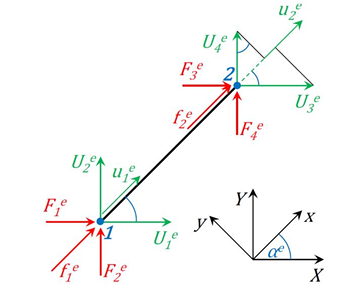
\includegraphics[width=\linewidth,height=0.55\textheight,keepaspectratio]{../Grafiken/V2_GlobaleElementmatrix.png}
    \end{column}
  \end{columns}
\end{frame}

\begin{frame}{Lernziele Vorlesung}
  \small
  Sie können
  \begin{enumerate}
    \item die lokale Elementsteifigkeitsmatrix $\mathbf{k}^e$ ($f^e=\mathbf{k}^eu^e$) für ein Feder und ein Stabelement aufstellen,
    \item unterscheiden zwischen
      \begin{itemize}
        \item lokalen Elementverschiebungen $u_i^e$ / Elementkräften $f_i^e$ ($i=1,2$),
        \item globalen Elementverschiebungen $U_j^e$ / Elementkräften $F_j^e$ ($j=1,\dots,4$),
        \item Strukturverschiebungen $U_l$ / Strukturkräften $F_l$ ($l=1,\dots,n$),
      \end{itemize}
    \item Elementverschiebungen und Elementkräfte vom lokalen ins globale System transformieren.
  \end{enumerate}
\end{frame}

\end{document}